\section{Simulation and user interface}
\label{sec:simulation}

\subsection{The automaton}

\code{CellularAutomaton} is the composition announced by the subject: a grid, a rule and a
discrete clock. One call to \code{step()} is one tick:

\begin{lstlisting}
public StepReport step() {
    int changed = grid.evolve(cell -> rule.nextState(grid, cell));
    generation++;
    if (changed == 0) {
        regime = Regime.FIXED_POINT;
    } else {
        int period = cycles.observe(grid.fingerprint(), generation);
        regime = period >= 2 ? Regime.cycle(period) : Regime.TRANSIENT;
    }
    return new StepReport(generation, changed, regime);
}
\end{lstlisting}

The automaton depends on the one-method interface \code{Rule}, not on the rule language: the
tests drive it with lambdas, and the expression trees of \cref{sec:rules} are plugged in through
the adapter \code{ExpressionRule}.

Section 1.2 of the subject describes two long-term behaviors: the grid may become ``identical
between two time steps'' (the automaton has \emph{converged}), or show ``periodic patterns that
repeat''. The automaton detects both and reports them as its \code{Regime}. Convergence is a step
that changed no cell. For cycles, a \code{CycleDetector} remembers a 64-bit fingerprint of each
of the last 1\,024 generations; since the evolution is deterministic, meeting a known fingerprint
again means that the automaton has entered a cycle whose period is the distance between the two
sightings. Remembering fingerprints rather than grids costs eight bytes per generation whatever
the size of the grid. On the \code{glider.xml} example, a glider travelling on a
$20 \times 20$ torus, the window announces a ``cycle of period 80'' at generation 80.

\subsection{Threading model}

A generation of a large grid takes tens of milliseconds, and a user interface must never wait
that long. The automaton therefore does not run on the Swing thread. \code{Simulation} owns one
background thread and \emph{confines} the automaton to it (\cref{fig:threads}):

\begin{itemize}
  \item every public method (\code{play}, \code{pause}, \code{step}, \code{reset},
    \code{setCell}, \code{setSlice}, \ldots) merely posts a command to that thread and returns;
  \item commands are executed one after the other, in order, so no lock is needed anywhere;
  \item nothing mutable leaves the thread: after each change the simulation publishes a
    \code{Snapshot}, an immutable record holding the generation, the population, the regime and
    the picture to display.
\end{itemize}

\begin{figure}[H]
  \centering
  \begin{tikzpicture}[
      lane/.style={draw=muted, fill=packfill, rounded corners=3pt, minimum width=5.4cm,
        minimum height=3.5cm},
      item/.style={draw=ink!60, fill=classfill, rounded corners=2pt, font=\ttfamily\scriptsize,
        inner sep=4pt, align=center},
      flow/.style={-{Straight Barb[length=3pt]}, line width=0.6pt, draw=ink!80},
      note/.style={font=\sffamily\scriptsize, text=muted, align=center}]
    \node[lane] (edt) at (0, 0) {};
    \node[lane] (sim) at (9.4, 0) {};
    \node[packagelabel, anchor=south west] at (edt.north west) {event dispatch thread (Swing)};
    \node[packagelabel, anchor=south west] at (sim.north west) {simulation thread};
    \node[item] (frame) at (0.4, 0.9) {SimulationFrame};
    \node[item] (canvas) at (0.4, -0.9) {FrameCanvas};
    \node[item] (simulation) at (8.2, 0) {Simulation};
    \node[item] (automaton) at (10.5, 0.9) {CellularAutomaton};
    \node[item] (projection) at (10.5, -0.9) {Projection};
    \draw[flow] (frame) -- (canvas);
    \draw[flow] (simulation.east) -- ++(0.35, 0) |- (automaton.west);
    \draw[flow] (simulation.east) -- ++(0.35, 0) |- (projection.west);
    \draw[flow] (frame.east) -- node[note, above, sloped] {commands: play, step, setCell, \dots}
      ($(simulation.west)+(0,0.12)$);
    \draw[flow] ($(simulation.west)+(0,-0.12)$) -- node[note, below, sloped]
      {immutable snapshots (latest wins)} (canvas.east);
  \end{tikzpicture}
  \caption{Threading model. The automaton and its grid are only ever touched by the simulation
    thread; the two threads exchange commands in one direction and immutable snapshots in the
    other.}
  \label{fig:threads}
\end{figure}

The window is an Observer of the simulation. Its listener is called on the simulation thread and
does one thing: hand the snapshot to the event dispatch thread. If snapshots arrive faster than
Swing can paint, the intermediate ones are dropped and only the latest is shown, so a simulation
running flat out never floods the interface:

\begin{lstlisting}
private void enqueue(Snapshot snapshot) {              // called on the simulation thread
    if (pending.getAndSet(snapshot) == null) {
        SwingUtilities.invokeLater(this::showPending);
    }
}
\end{lstlisting}

\begin{figure}[tbp]
  \centering
  \begin{tikzpicture}
    \node[class=3] (sim) at (0, 0) {\ctitle{Simulation}
      \nodepart{second}- worker: ScheduledExecutorService\\- running: boolean\\
        - intervalMillis: long
      \nodepart{third}+ play() / pause() / step()\\+ reset() / reseed() / clear()\\
        + setCell(row, column, state)\\+ setSlice(slice)\\+ setInterval(millis)\\
        + addListener(listener)\\+ state(): CompletableFuture<Snapshot>\\+ close()};
    \node[iface] (listener) at (-4.7, 1.4) {\ctitle[interface]{SimulationListener}
      \nodepart{second}+ simulationChanged(snapshot)};
    \node[class] (snapshot) at (-4.7, -1.6) {\ctitle[record]{Snapshot}
      \nodepart{second}+ generation: long\\+ population: int\\+ changedCells: int\\
        + regime: Regime\\+ running: boolean\\+ frame: Frame};
    \node[class=3] (automaton) at (5.2, 1.2) {\ctitle{CellularAutomaton}
      \nodepart{second}- generation: long
      \nodepart{third}+ step(): StepReport\\+ advance(steps)\\+ restart(initializer)\\
        + regime(): Regime};
    \node[class] (cycles) at (8.1, -1.5) {\ctitle{CycleDetector}
      \nodepart{second}\textasciitilde{} observe(...): int\\\textasciitilde{} reset()};
    \node[class] (regime) at (4.7, -1.6) {\ctitle[record]{Regime}
      \nodepart{second}+ kind: Kind\\+ period: int};
    \node[iface] (projection) at (2.2, -4.3) {\ctitle[interface]{Projection}
      \nodepart{second}+ restarted(grid)\\+ advanced(grid)\\+ edited(grid)\\+ frame(grid): Frame\\
        + locate(row, column): Coordinates};
    \node[class] (plane) at (6.2, -3.9) {\ctitle{PlaneProjection}\nodepart{second}- slice: Slice};
    \node[class] (spacetime) at (6.7, -5.3) {\ctitle{SpaceTimeProjection}
      \nodepart{second}- rows: Deque<int[]>};

    \draw[aggregation] ($(sim.west)+(0,1.4)$) -- node[elabel, above] {notifies} (listener.east);
    \draw[uses] ($(sim.west)+(0,-1.2)$) -- node[elabel, above] {publishes}
      (snapshot.east |- {$(sim.west)+(0,-1.2)$});
    \draw[uses] (listener) -- (snapshot);
    \draw[composition] ($(sim.east)+(0,1.2)$) -- (automaton.west |- {$(sim.east)+(0,1.2)$});
    \draw[composition] (automaton.east) -| (cycles.north);
    \draw[association] (automaton.south -| regime.north) -- (regime.north);
    \draw[composition] (sim.south -| projection.north) -- (projection.north);
    \draw[implements] (plane.west) -- (plane.west -| projection.east);
    \draw[implements] (spacetime.west) -- ++(-0.6, 0) |- ($(projection.east)+(0,-0.6)$);
  \end{tikzpicture}
  \caption{The \code{automaton} and \code{simulation} packages.}
  \label{fig:simulation}
\end{figure}

\subsection{From a grid to a picture}

The subject asks for two displays. \code{Projection} is the interface behind both, a Strategy
chosen from the dimension of the grid:

\begin{itemize}
  \item \code{SpaceTimeProjection}, for one dimension, keeps the last 1\,024 generations and
    stacks them: this is the ``juxtaposition of successive states'' in which rule 18 draws the
    Sierpi\'nski triangle;
  \item \code{PlaneProjection}, for two dimensions and more, shows the current generation
    through a \code{Slice}, which can be moved while the simulation runs.
\end{itemize}

Both produce a \code{Frame}. The window, the PNG export and the text output all draw frames, so
the three share one rendering path and the exported picture is exactly what was on screen.

\subsection{The windows}

The interface is written with Swing and consists of two windows.

The \textbf{menu} (\cref{fig:launcher}) is the start-up screen required by the subject. It lists
the definition files of the current directory, or of another one, with what each describes.
Invalid files are listed in red with the reason of their rejection.

\begin{figure}[H]
  \centering
  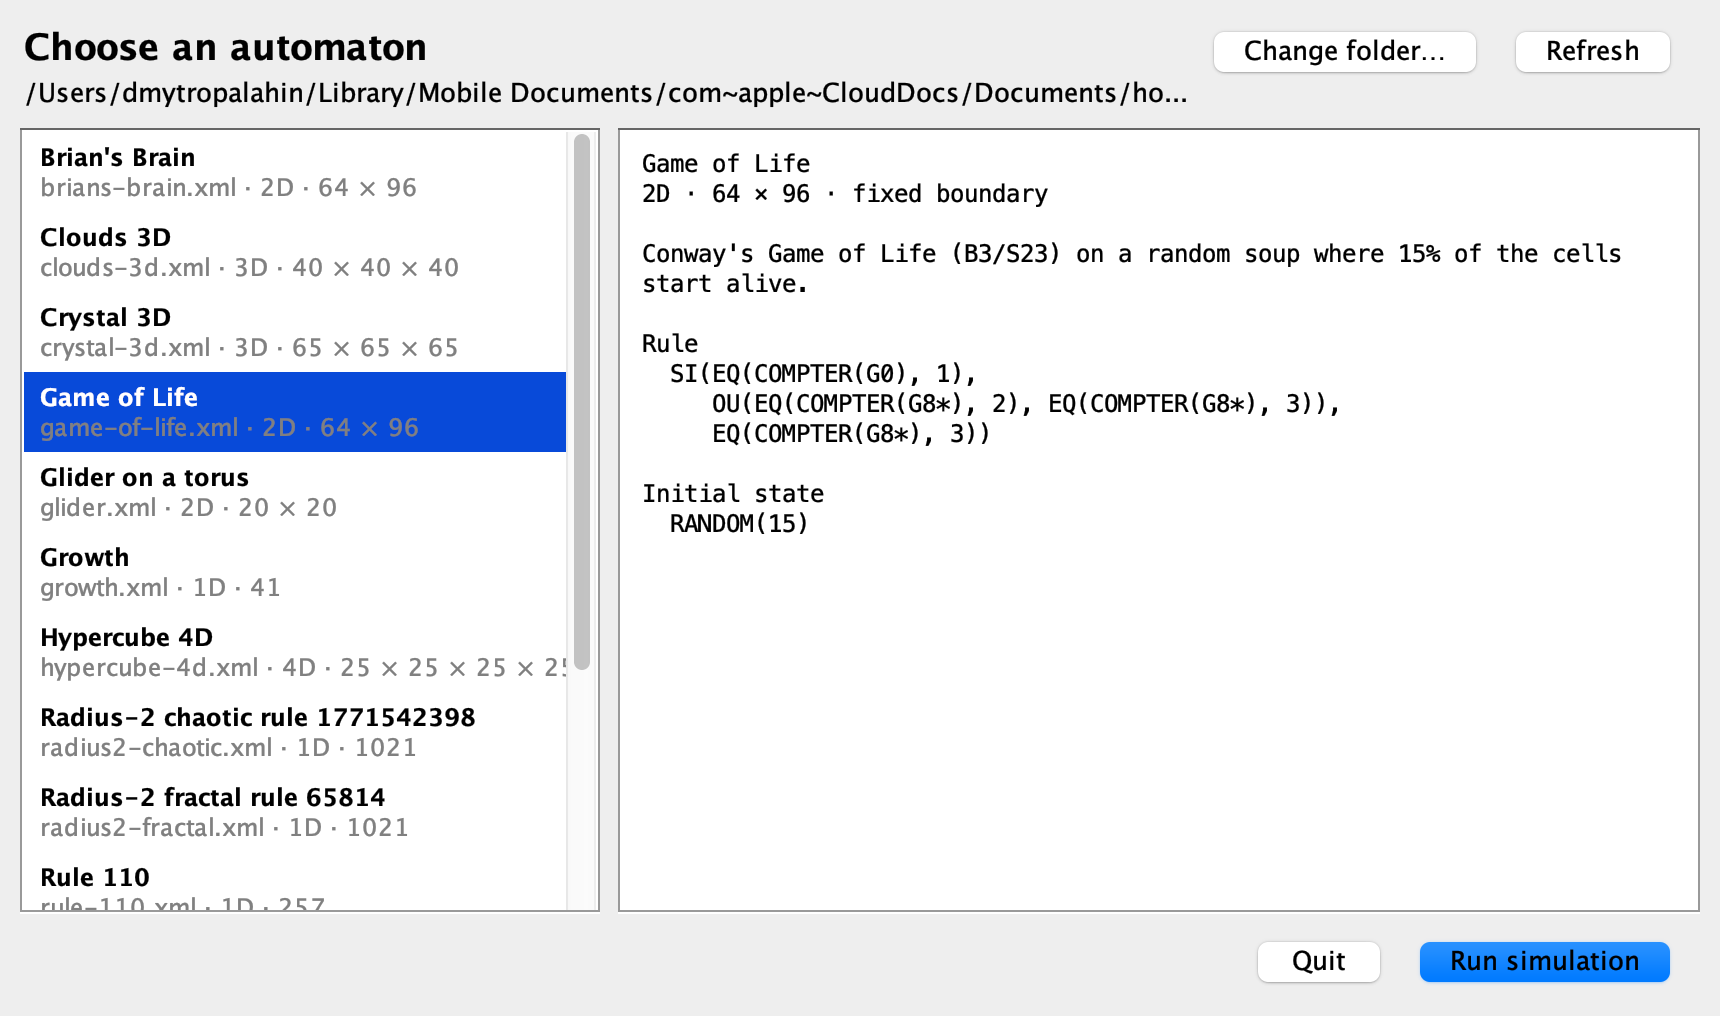
\includegraphics[width=0.74\textwidth]{launcher}
  \caption{The menu of the definition files of a directory.}
  \label{fig:launcher}
\end{figure}

The \textbf{simulation window} (\cref{fig:window}) shows one automaton. A toolbar gives the
commands (play or pause, single step, reset, new random draw, clear, speed, PNG export), a status
bar gives the generation, the population, the number of cells changed by the last step and the
regime. Clicking or dragging on the picture switches cells on and off, which makes it easy to
try a glider by hand. For a grid of three dimensions or more, a bar shows the slice in the
notation of the subject, with one spinner per pinned axis to move the plane.

\begin{figure}[H]
  \centering
  \begin{subfigure}[b]{0.43\textwidth}
    \centering
    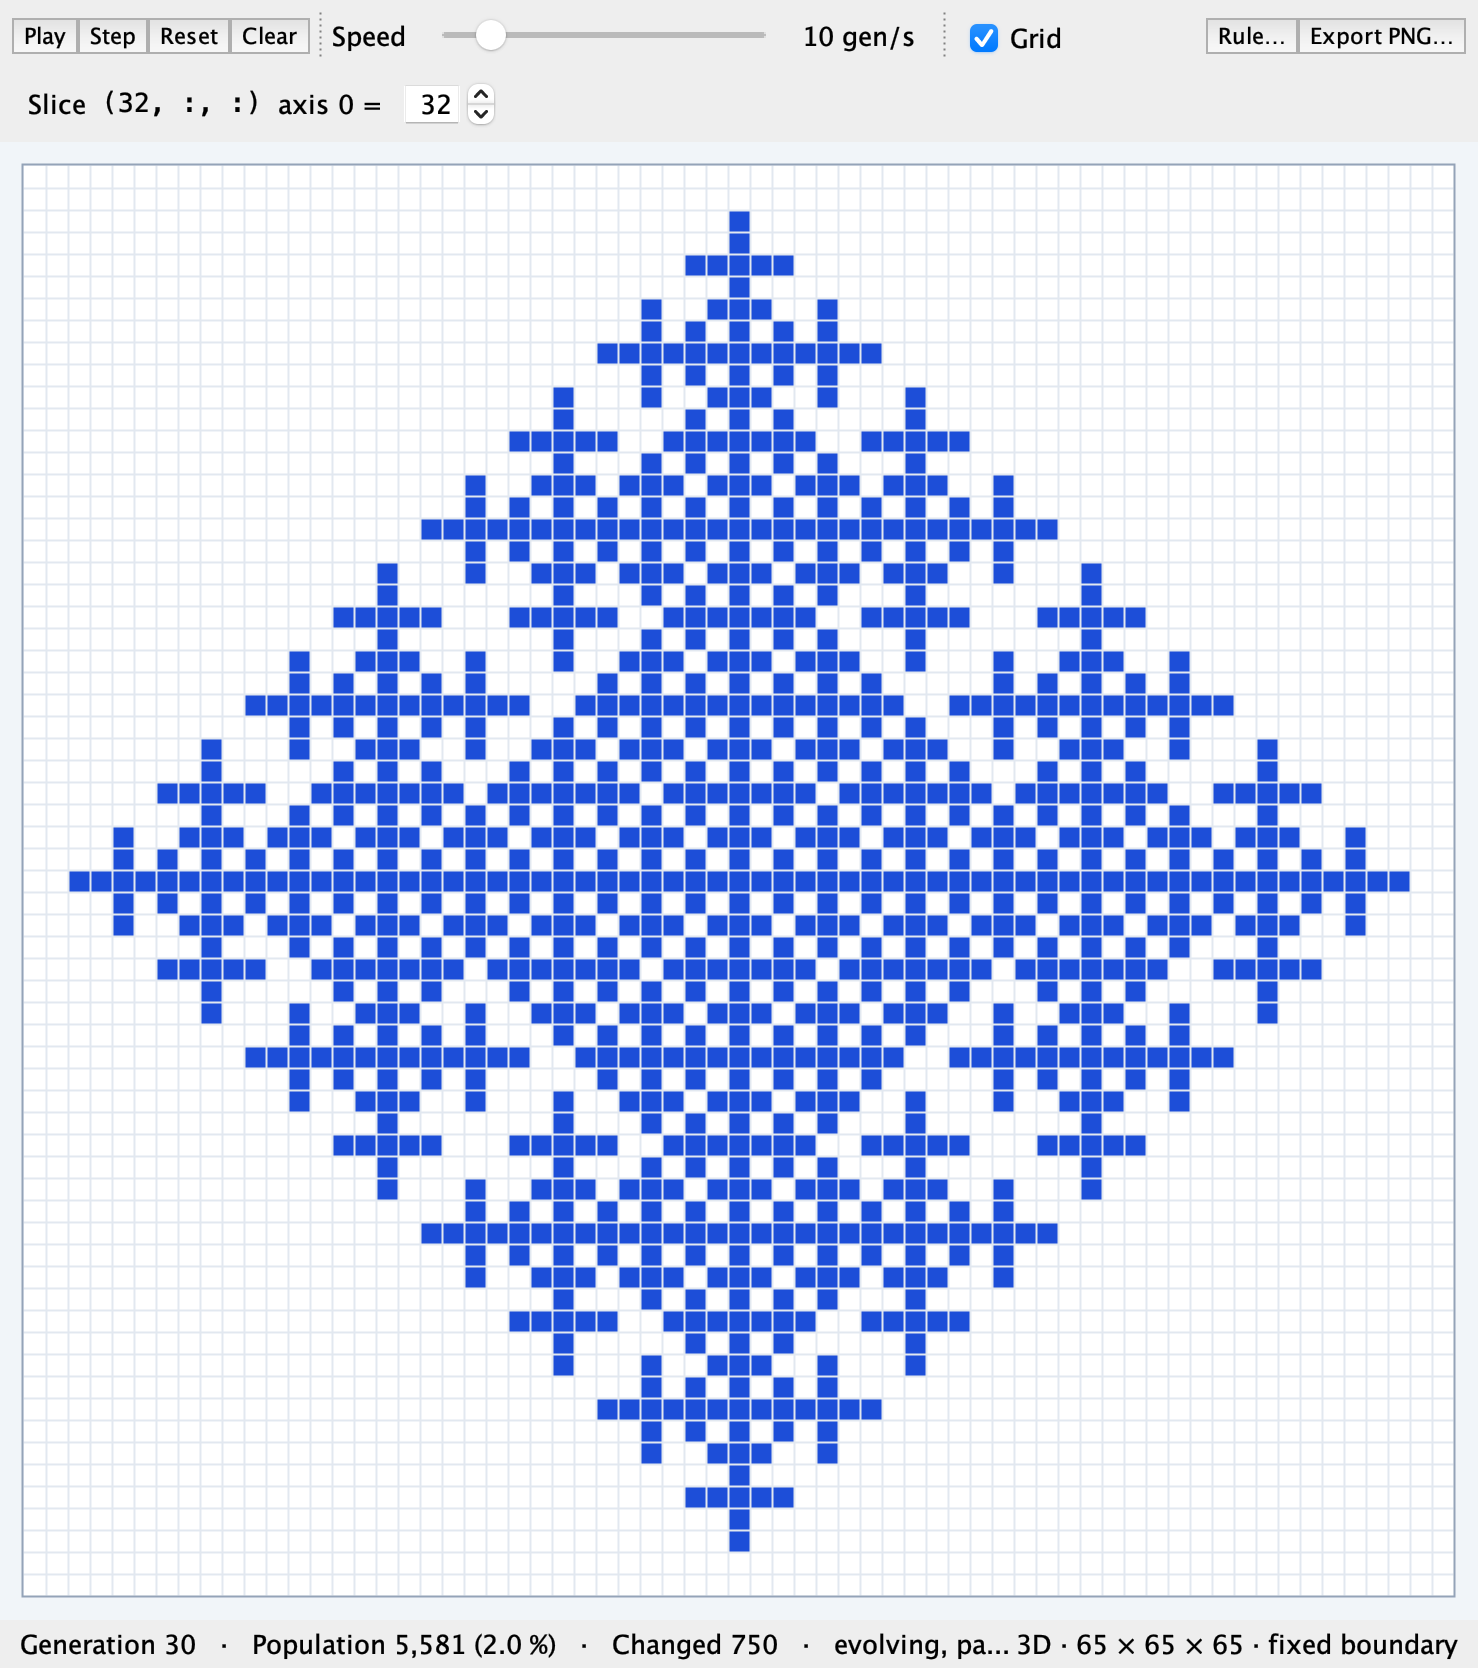
\includegraphics[width=\textwidth]{window-crystal-3d}
    \caption{A 3D automaton seen through the plane \code{(32, :, :)}}
  \end{subfigure}\hfill
  \begin{subfigure}[b]{0.55\textwidth}
    \centering
    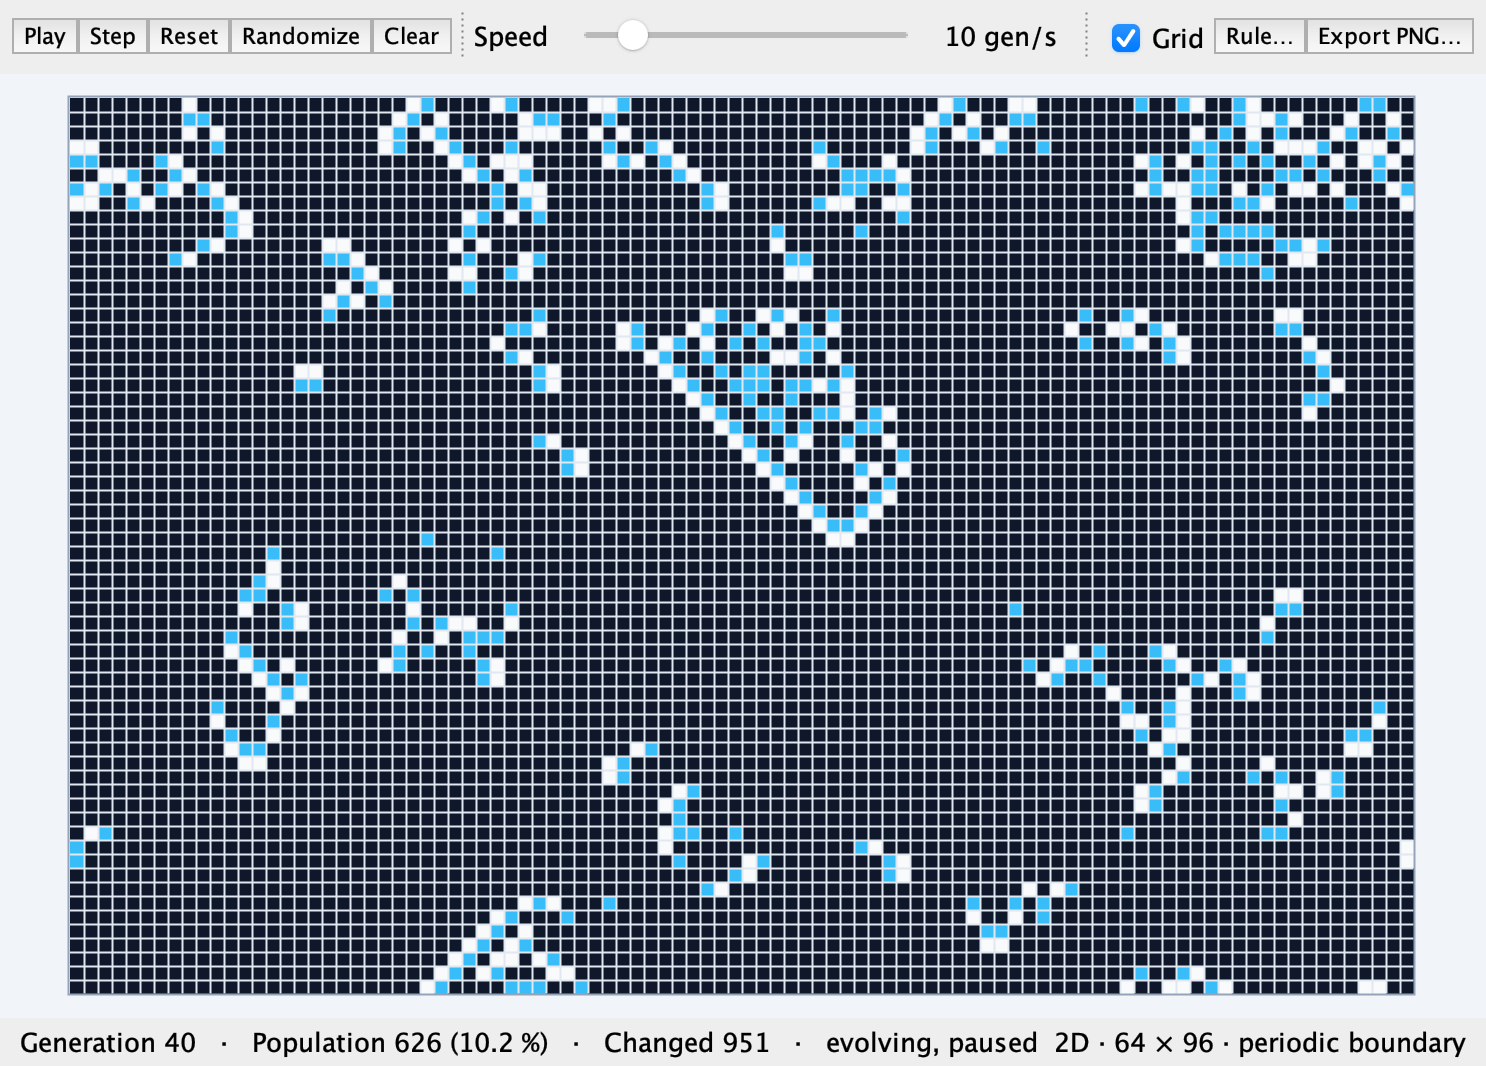
\includegraphics[width=\textwidth]{window-brians-brain}
    \caption{Brian's Brain, a three-state automaton with custom colors}
  \end{subfigure}
  \caption{The simulation window.}
  \label{fig:window}
\end{figure}

The drawing itself is done by \code{FrameCanvas}. A frame is first rendered at one pixel per
cell into an image, with a table lookup per cell, then magnified by the graphics library with
nearest-neighbor interpolation. Repainting a million cells is thus one array pass and one image
blit.

\subsection{Without a display}

Everything the windows do is also available from the command line (\cref{tab:commands}), through
the same classes. The command-line interface is what made it possible to test the application end
to end on a build server, and to produce the figures of this report with the program itself.
When no display is available, the menu falls back to a numbered list in the terminal.

\begin{table}[H]
  \centering\small
  \begin{tabularx}{0.92\textwidth}{@{}l L@{}}
    \toprule
    Command & Effect \\
    \midrule
    \code{menu} (default) & List the definition files of a directory and launch one \\
    \code{run FILE} & Open the simulation window of one file \\
    \code{list}, \code{validate FILE...} & Print the files of a directory; check files and
      explain what is wrong \\
    \code{print FILE}, \code{render FILE} & Run an automaton and output the result as text, or as
      a PNG image \\
    \code{explore} & Search for fractal or chaotic rules of radius 2 (\cref{sec:bonus}) \\
    \bottomrule
  \end{tabularx}
  \caption{The commands of the application.}
  \label{tab:commands}
\end{table}
